\documentclass{book}

\usepackage[utf8]{inputenc}
\usepackage[T1]{fontenc}
\usepackage[francais]{babel}

% Define book information
\title{Le théorème de Pythagore}
\author{Jämes \textsc{Ménétrey}}
\date{\today}

% Define the theorems
\newtheorem{theoreme}{Théorème}
\newtheorem{reciproque}{Réciproque}

% Package for loading pictures
\usepackage{graphicx}

% Package for tables
\usepackage{array}

% Packages and definitions for colors
\usepackage{color}
\usepackage{colortbl}
\definecolor{grey}{RGB}{200,200,200}

% Package for the bibliography
% Arguments for biblatex available here: http://tex.stackexchange.com/a/52106/108649
\usepackage[backend=bibtex,style=numeric,sorting=none]{biblatex}
\addbibresource{bibliography.bib}

\begin{document}

% Change the name of the toc
\renewcommand{\contentsname}{Sommaire}

\maketitle

\frontmatter

\tableofcontents

\chapter{Introduction}

Le théorème de Pythagore est un théorème de géométrie euclidienne qui met en relation les longueurs des côtés dans un triangle rectangle : le carré de la longueur de l’hypoténuse, qui est le côté opposé à l'angle droit, est égal à la somme des carrés des longueurs des deux autres côtés.

Ce théorème permet notamment de calculer l’une de ces longueurs à partir des deux autres. Il est nommé d’après Pythagore \textsc{de Samos}, philosophe de la Grèce antique.

\begin{figure}[h]
\begin{center}
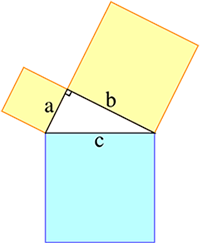
\includegraphics{img/intro.png}
\end{center}
\caption{Une version géométrique du théorème}
\label{Une version géométrique du théorème}
\end{figure}

\mainmatter

\part{Théorème de Pythagore}

\chapter{Enoncé du théorème}

\section{Théorie}

La forme la plus connue du théorème de Pythagore\cite{wiki2016pythagore} est la suivante :

\begin{theoreme}[de Pythagore]
Dans un triangle rectangle, le carré de la longueur de l’hypoténuse est égal à la somme des carrés des longueurs des côtés de l’angle droit.
\end{theoreme}

En particulier, la longueur de l’hypoténuse est donc toujours supérieure à celle de chaque autre côté.

Le terme « longueur » est parfois omis, chaque côté étant assimilé à sa longueur. Toutefois l’élévation au carré (algébrique), qui n’a de sens que pour une grandeur numérique comme la longueur, correspond à la construction d’un carré (géométrique) sur chaque côté du triangle. Certaines démonstrations du théorème s’appuient d’ailleurs sur une égalité d’aires entre le carré construit sur l’hypoténuse et la réunion des carrés construits sur les deux autres côtés.

En nommant les sommets du triangle, le théorème peut se reformuler dans l’implication suivante : Si un triangle $ABC$ est rectangle en $C$, alors $AB^{2} = AC^{2} + BC^{2}$.

\begin{figure}
\begin{center}
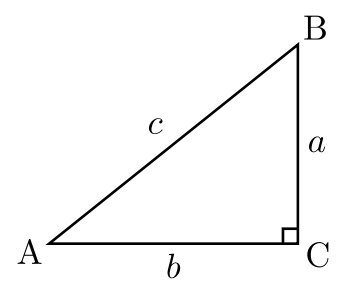
\includegraphics{img/exemple.png}
\end{center}
\caption{Triangle rectangle}
\label{Triangle rectangle}
\end{figure}

\section{Exemple}

Avec les notations ci-dessus, soit le triangle rectangle de côtés $a = 3$ et $b = 4$; alors la longueur du troisième côté $c$, est données par: $a^{2} + b^{2} = 32 + 42 = 25 = c^{2}$. Les longueurs étant des réels positifs, on obtient $c = 5$. Un triplet de nombres entiers tel que $(3, 4, 5)$, représentant la longueur des côtés d'un triangle rectangle s'appelle un triplet pythagoricien.

\chapter{Réciproque}

La réciproque du théorème de Pythagore est également vraie:

\begin{reciproque}[Théorème de Pythagore.]
Si dans un triangle, le carré de la longueur d'un côté est égal à la somme des carrés des longueurs des deux autres côtés, alors ce triangle est rectangle et son hypoténuse est le plus grand côté.
\end{reciproque}

Le théorème de Pythagore est donc une propriété caractéristique des triangles rectangles. Formulé autrement, si dans un triangle $ABC$ on a $BC^{2} + AC^{2} = AB^{2}$, alors ce triangle est rectangle en $C$.

\appendix

\part{Annexes et tables}

\chapter{Table d'addition}

Table issue de Wikipédia\cite{wiki2015addition}.

\begin{table}
\begin{center}
\begin{tabular}{| >{\begin{bf}\columncolor{grey}} c <{\end{bf}} |c|c|c|}
\hline
\rowcolor{grey}Additionné à & 1 & 2 & 3 \\
\hline
1 & 2 & 3 & 4 \\
\hline
2 & 3 & 4 & 5 \\
\hline
3 & 4 & 5 & 6 \\
\hline
\end{tabular}
\end{center}
\caption{Table d'addition}
\label{Table d'addition}
\end{table}

\chapter{Table de multiplication}

Table issue de Wikipédia\cite{wiki2015multiplication}.

\begin{table}
\begin{center}
\begin{tabular}{| >{\begin{bf}\columncolor{grey}} c <{\end{bf}} |c|c|c|}
\hline
\rowcolor{grey}Multiplié à & 1 & 2 & 3 \\
\hline
1 & 1 & 2 & 3 \\
\hline
2 & 2 & 4 & 6 \\
\hline
3 & 3 & 6 & 9 \\
\hline
\end{tabular}
\end{center}
\caption{Table de multiplication}
\label{Table de multiplication}
\end{table}

\backmatter

\listoffigures
\listoftables

\printbibliography
	
\end{document}